% !TEX root = comparison.tex
\section{Experimental Setup}
We want two discuss two applications, in which we are making use of lineups to compare competing designs. 
The first one arises from a discussion of how wind direction affects efficiency of an airport. In this example, we are dealing with all flights \cite{rita} in and out of Seattle/Tacoma International Airport (SEA) between July 2008 and June 2011. As a measure of airport efficiency we are using time between successive wheel-events (time at wheel take-off or touch-down), which we found to be independent of airline carrier and operating hours, as long as we restricted the data to `regular' operating hours between 7 am and midnight and `regular' weather conditions -- i.e. we eliminated records associated with the top 5\% wind speed measurements \cite{noaa-weather}, leaving us with just under 0.5 Million flights.

Statistical tests of mean efficiency by wind direction are not particularly helpful in this situation:
the difference in mean efficiency between the most efficient wind direction and the least efficient shows a statistically significant difference with a $p$-value $\le 10^{15}$. %2.2e-16$. 
However, out of the 34 other wind directions,  another 31 show significant differences in efficiency as well. This is much more a property of the large data size rather than practically usable differences. Mere significances also do not allow us an assessment of the underlying pattern.

\subsection{Wind Direction and Airport Efficiency}
In deciding on the design for displaying efficiency  by wind direction we were using the fact that wind direction is circular, and  displayed the data as (conditional) wind rose charts - i.e. for each of 36 wind directions we show the percentage of flights falling into one-minute intervals between successive flights, from  0 minutes to 8 minutes or more.


\begin{figure}[htbp] %  figure placement: here, top, bottom, or page
%   \centering
 \hspace{-.1in}
   \begin{tabular}{ccl}
   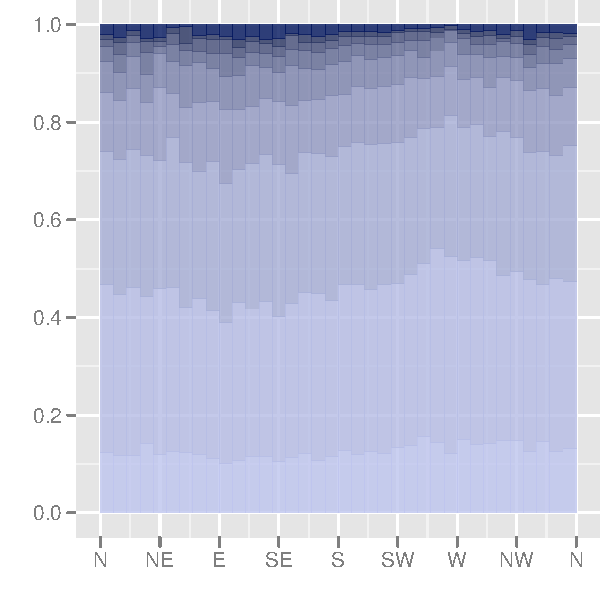
\includegraphics[width=0.375\linewidth]{euclid_noline.pdf} & \hspace{-.3in}
   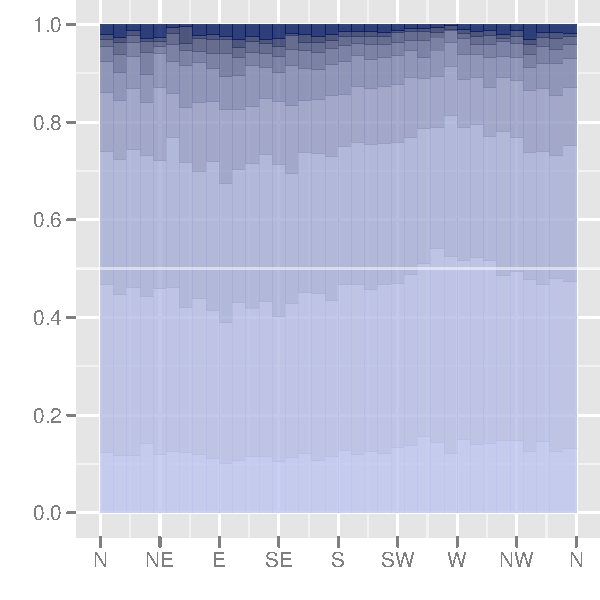
\includegraphics[width=0.375\linewidth]{euclid_line.pdf} &  \hspace{-.2in} \multirow{2}{*}[.55in]{  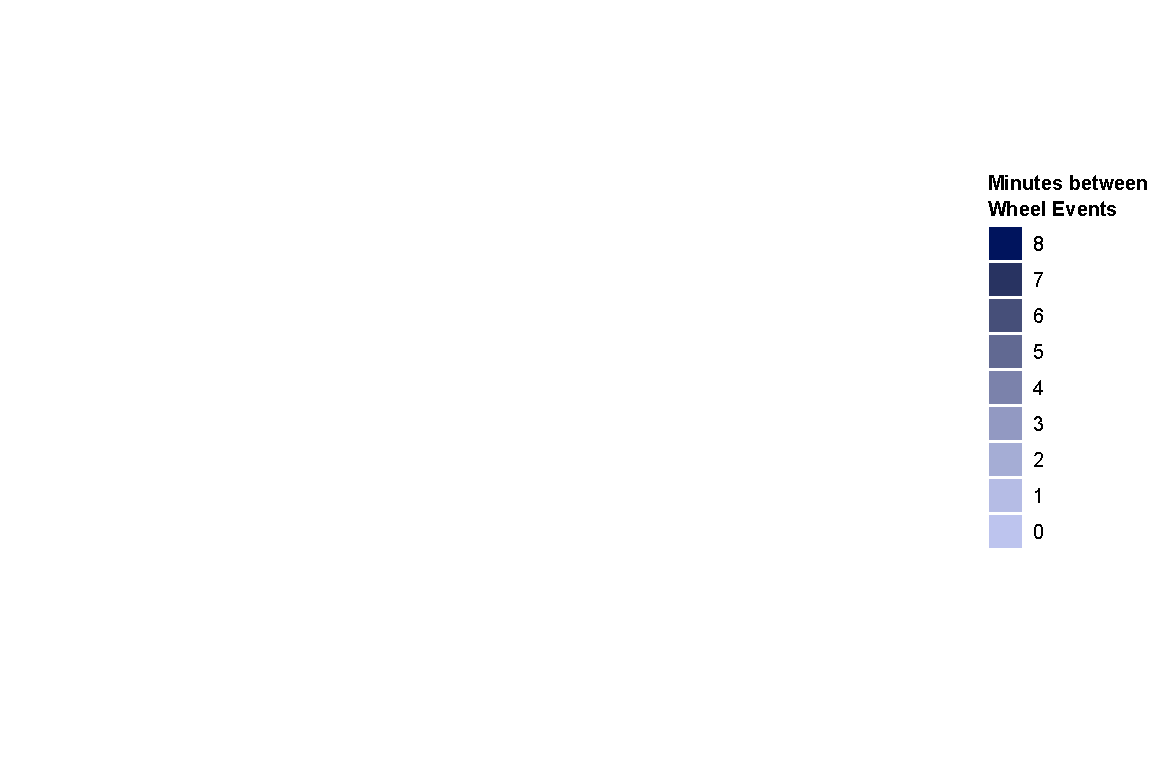
\includegraphics[width=0.2\linewidth]{legend.pdf}} \\
   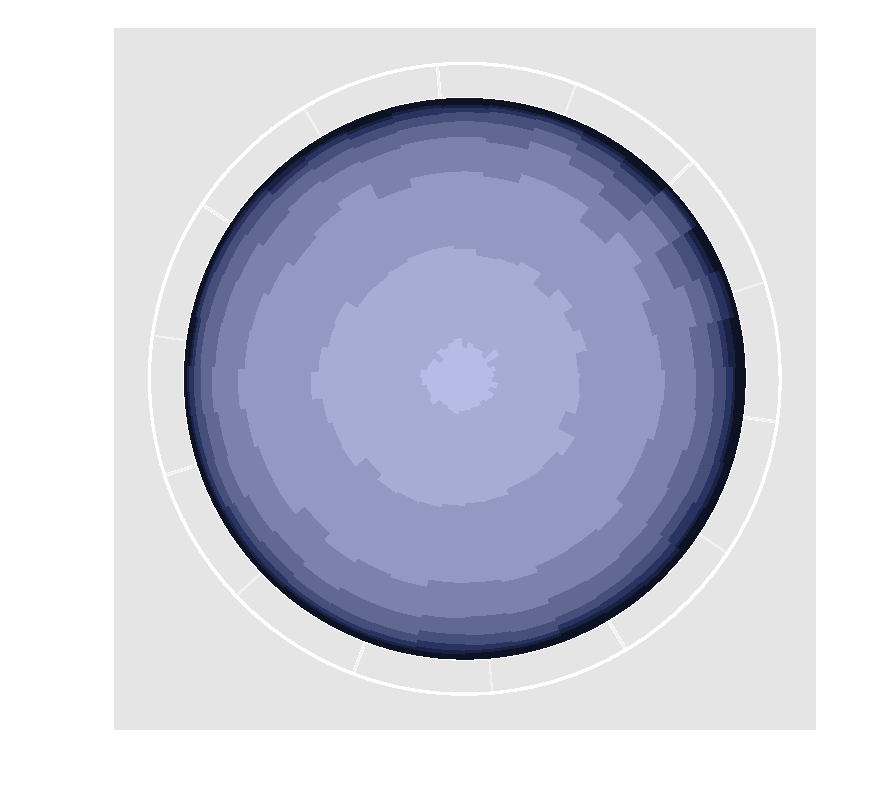
\includegraphics[width=0.43\linewidth]{Polar_NoLine.pdf} &  \hspace{-.3in}
   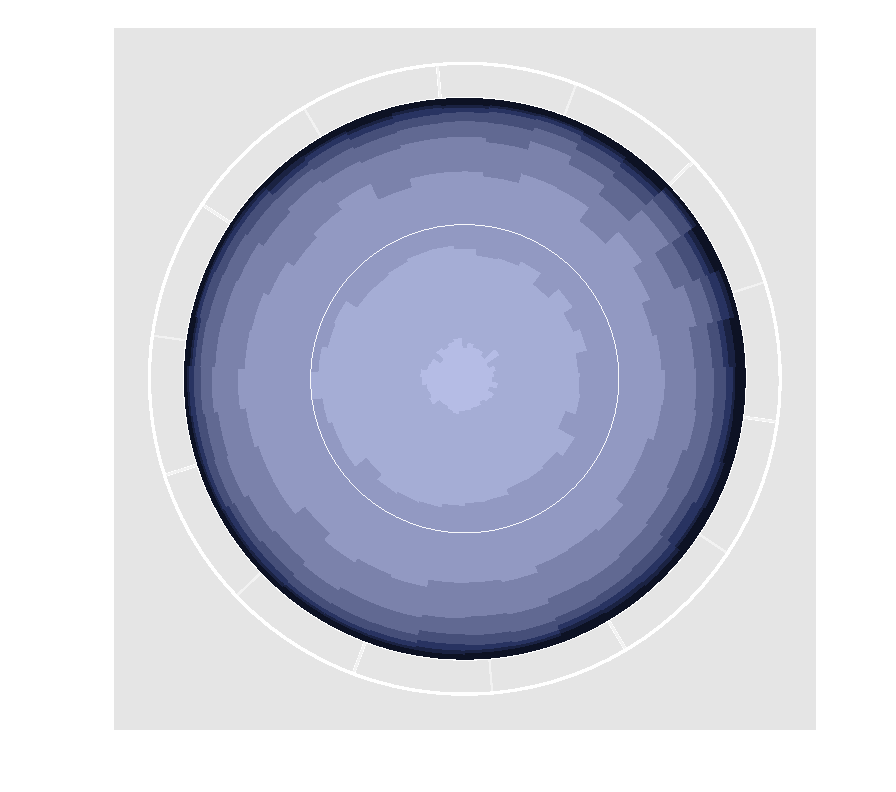
\includegraphics[width=0.43\linewidth]{Polar_Line.pdf}  
   \end{tabular}
   \caption{All four competing designs: polar versus Euclidean charts in top and bottom row, with (right) and without (left) reference lines at 50\%. }
   \label{layouts}
\end{figure}

In spite of the contextual circular property of wind direction, the pattern in efficiency did not seem to stand out well during the exploration process, which led us to using a corresponding  Euclidean design. Both designs were additionally equipped with a reference line at 50\%. 
Figure \ref{layouts} shows an overview of all four chart types in the study. During the exploration of the data, it became clear that Seattle airport functions at it best with winds coming from the East to Southeast, while winds from the West seemed to be most troublesome, resulting in a wave-like pattern in the Euclidean charts and a shift in center for the polar charts. Since runways can be used in both directions, changing the runway usage according to dominant wind direction for that day or time of the year might be a feasible solution in gaining efficiency. 

\begin{figure}[htbp] %  figure placement: here, top, bottom, or page
   \centering

\begin{tabular}{cl}
\phantom{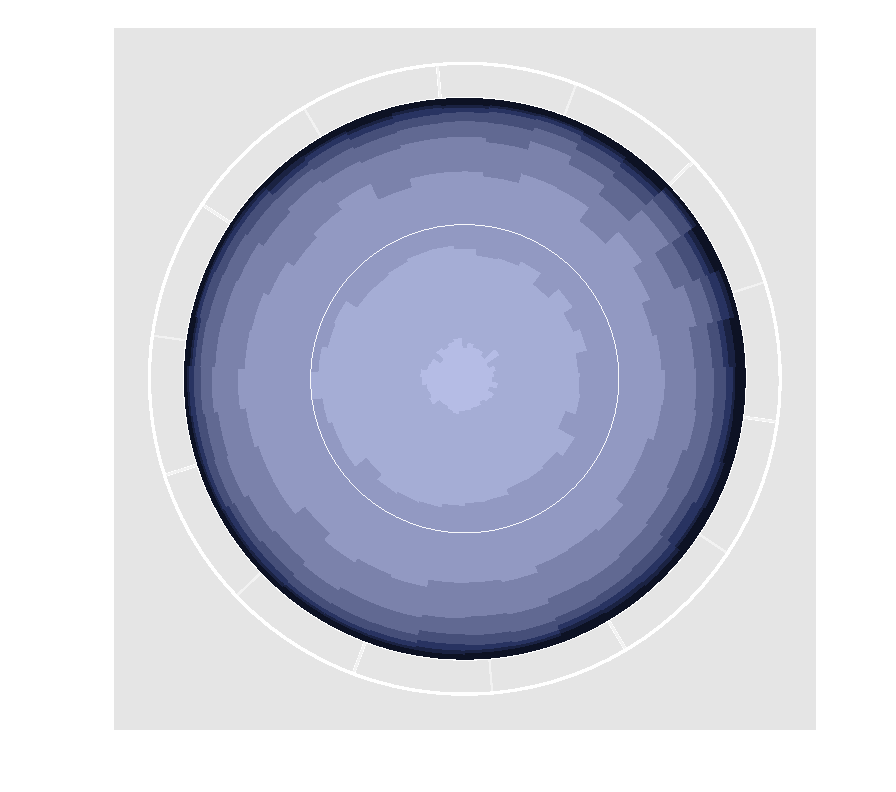
\includegraphics[width=0.03\linewidth]{Polar_Line.pdf}} & \vspace{-0.035in} \multirow{10}{*}{\hspace{-0.25in}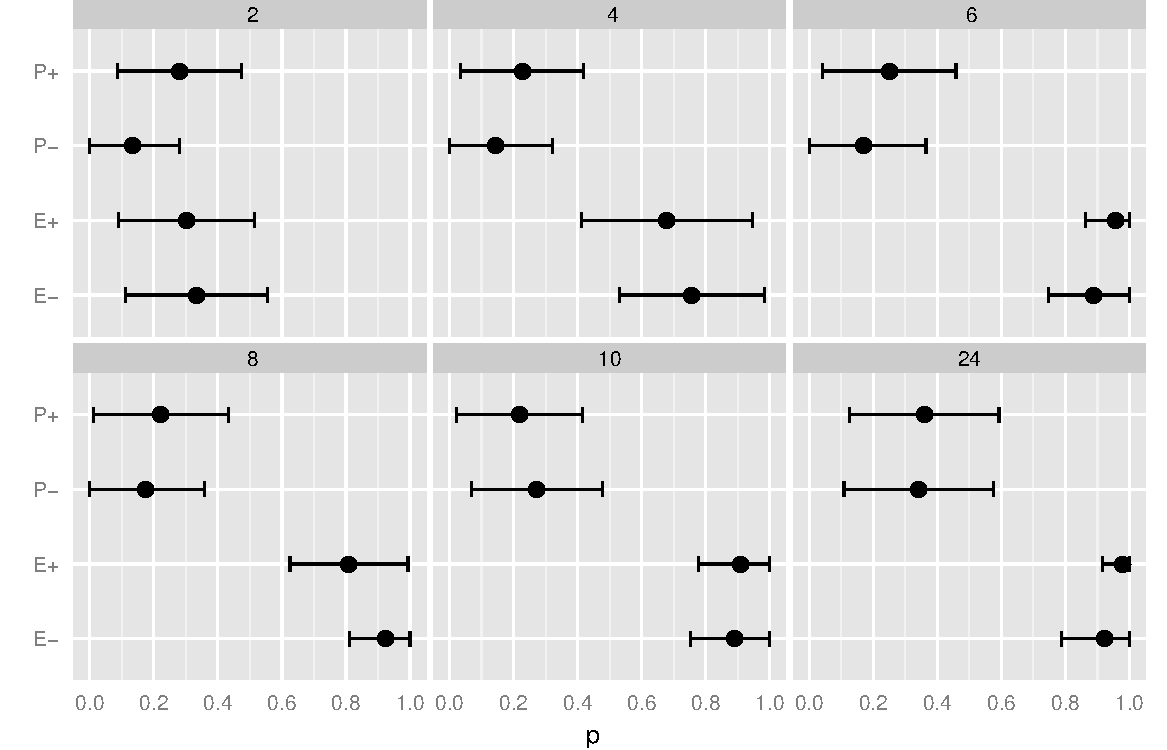
\includegraphics[width=0.9\linewidth]{turk4-designs.pdf}} \\
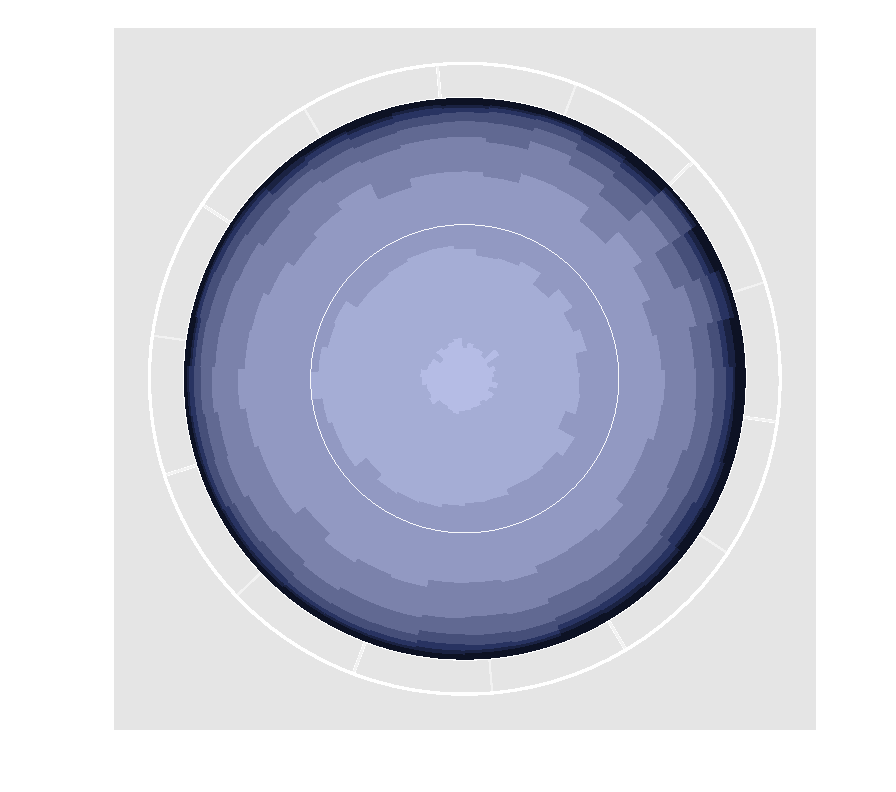
\includegraphics[width=0.05\linewidth]{Polar_Line.pdf} \\
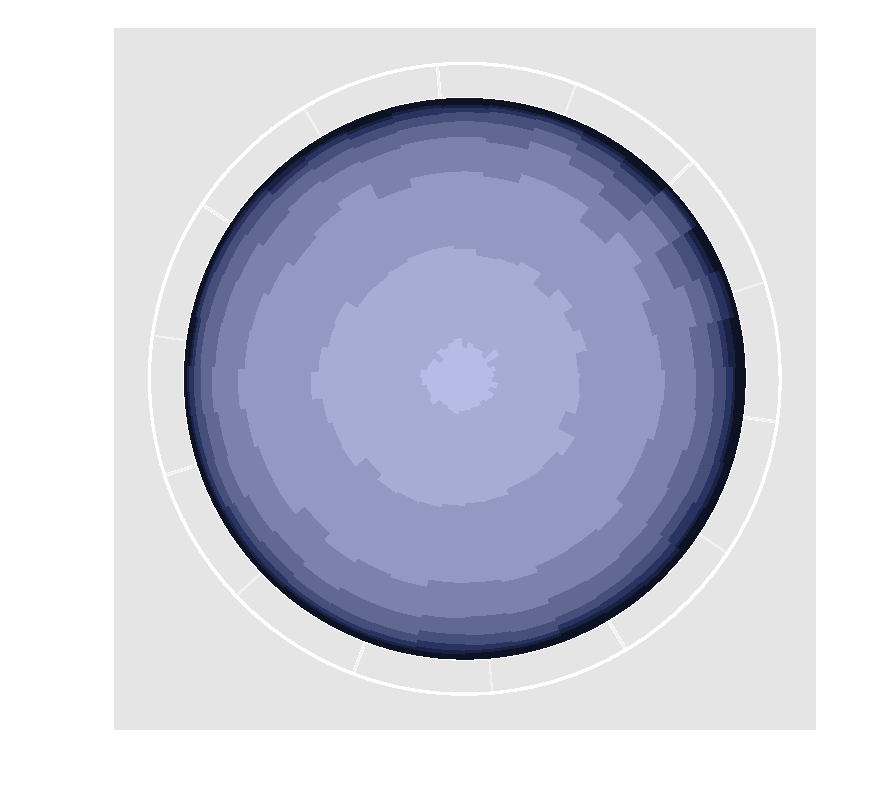
\includegraphics[width=0.05\linewidth]{Polar_NoLine.pdf} \\
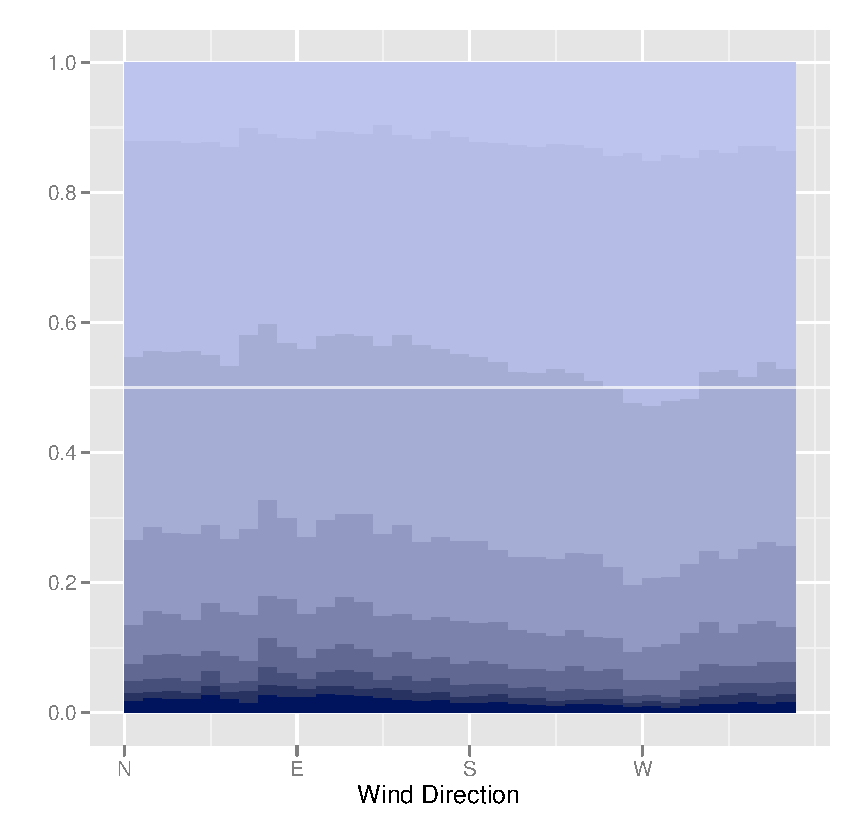
\includegraphics[width=0.043\linewidth]{Euclidian_Line.pdf} \\
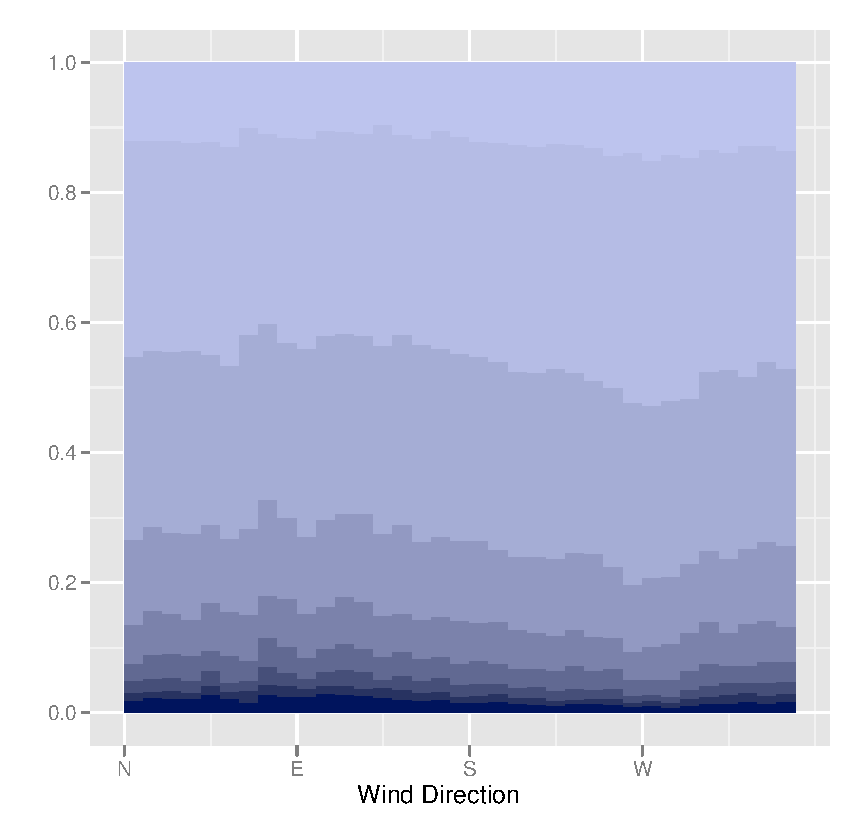
\includegraphics[width=0.043\linewidth]{Euclidian_NoLine.pdf}\\
\phantom{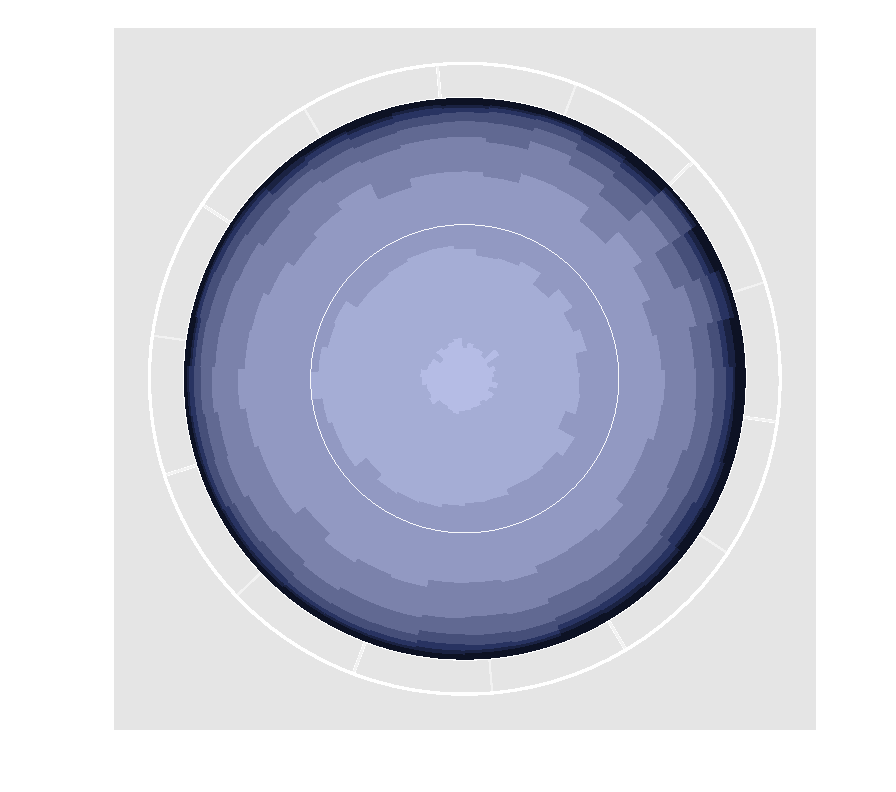
\includegraphics[width=0.015\linewidth]{Polar_Line.pdf}}\\
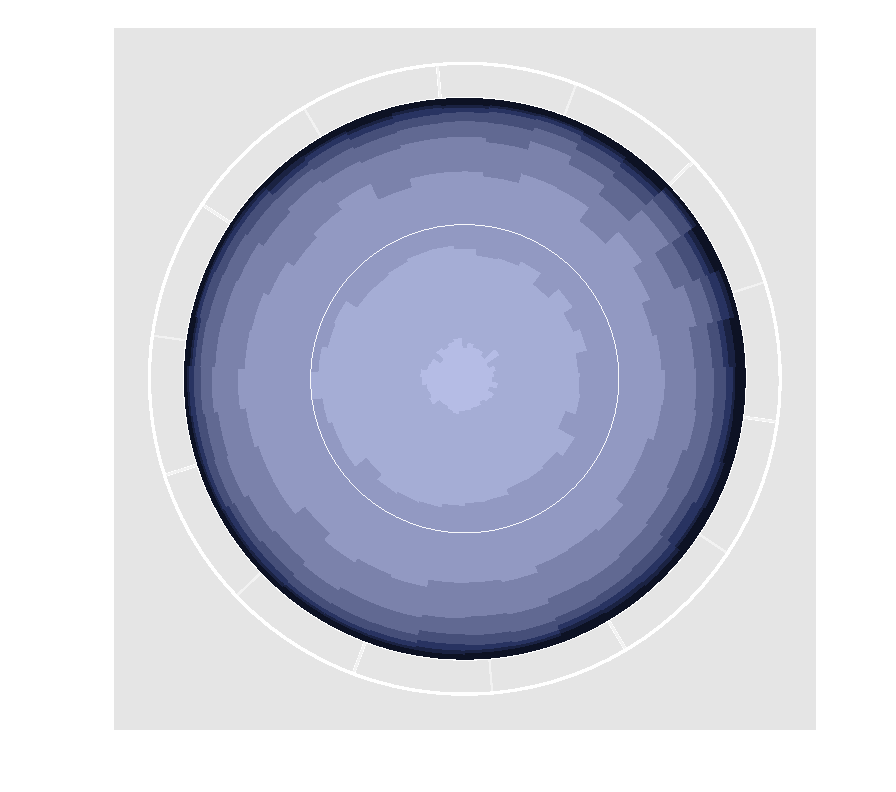
\includegraphics[width=0.05\linewidth]{Polar_Line.pdf} \\
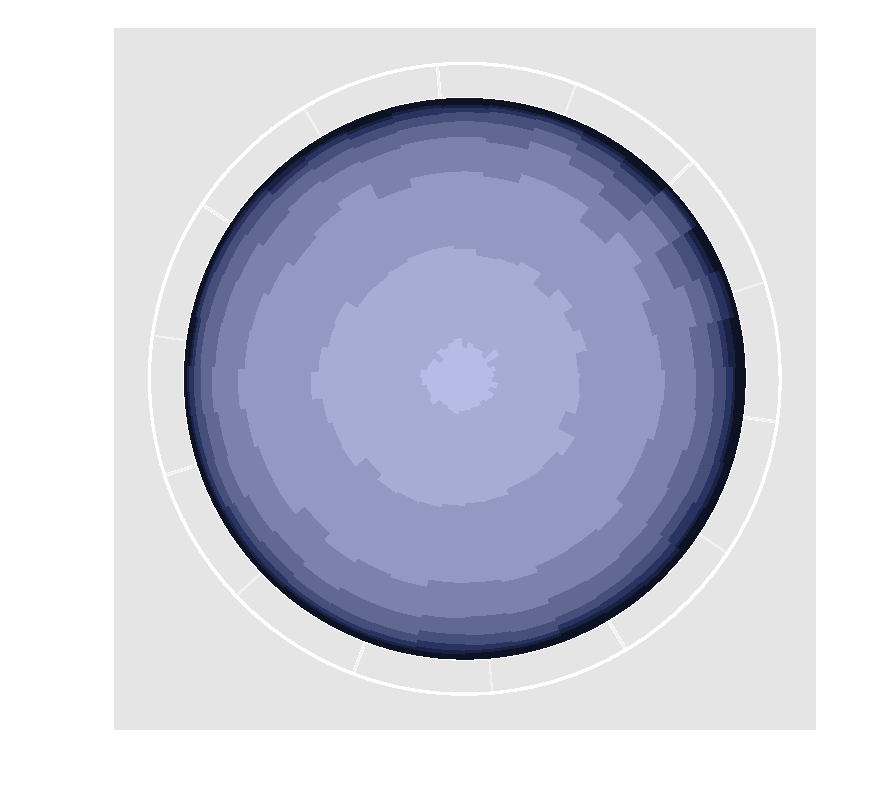
\includegraphics[width=0.05\linewidth]{Polar_NoLine.pdf} \\
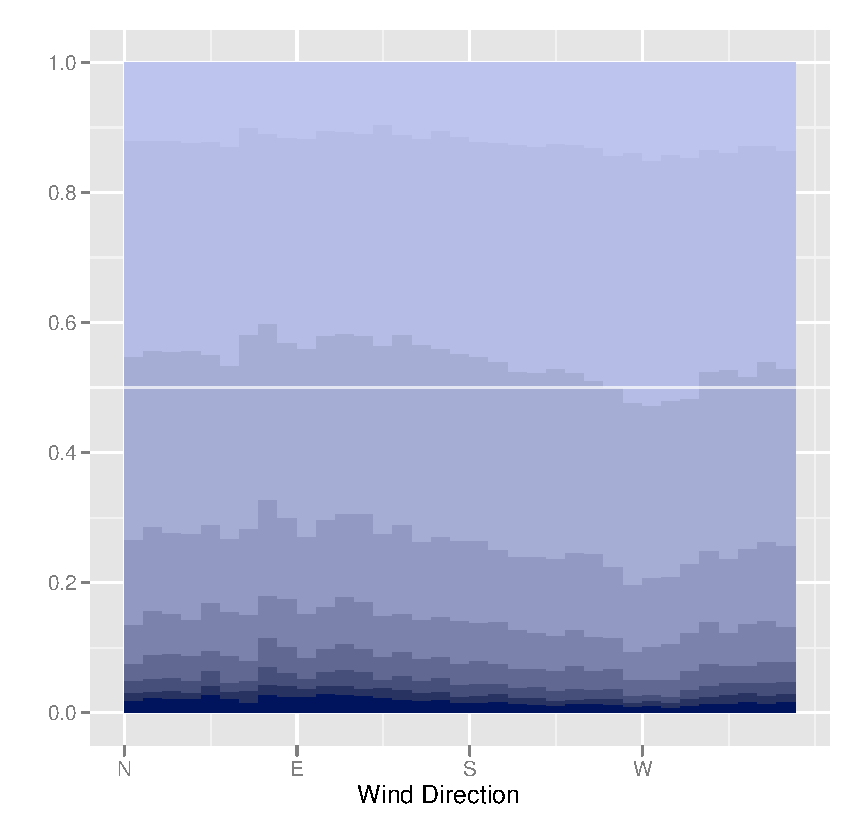
\includegraphics[width=0.043\linewidth]{Euclidian_Line.pdf} \\
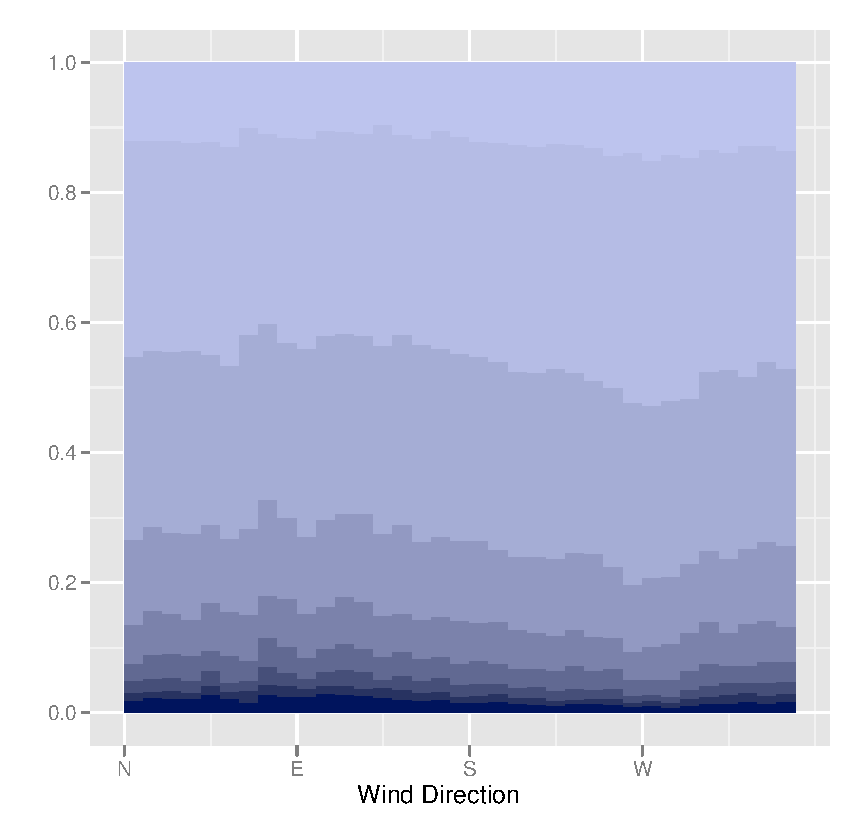
\includegraphics[width=0.043\linewidth]{Euclidian_NoLine.pdf}\\
  \end{tabular} 
  \vspace{0.1in}
   \caption{Power results for two competing designs: polar versus a Euclidean, with and without a reference line. Error bars indicate 95\% confidence intervals. Plots are facetted by percentage of data used. }
   \label{fig:treatment}
\end{figure}

An additional factor we were interested in this particular situation was to assess, how much of the data we actually needed to use in a design to have observers pick out the pattern. Clearly, a design is more efficient, if a smaller sample size is sufficient for showing the presence of a relationship. In order to investigate this, we took different size samples of the data and created lineup plots of all four designs for these subsets. The effect of sampling size on the displays mostly stems from the additional variability introduced when using small samples, which might hide the pattern, if it is not displayed prominently. 
XXX picture of sampling size?
Another perturbation to the data are `shifts' in wind direction, i.e. we make use of the circular nature of the wind direction and adjust the $x$ axis by using different offsets.

\begin{figure}[htbp] %  figure placement: here, top, bottom, or page
   \centering
   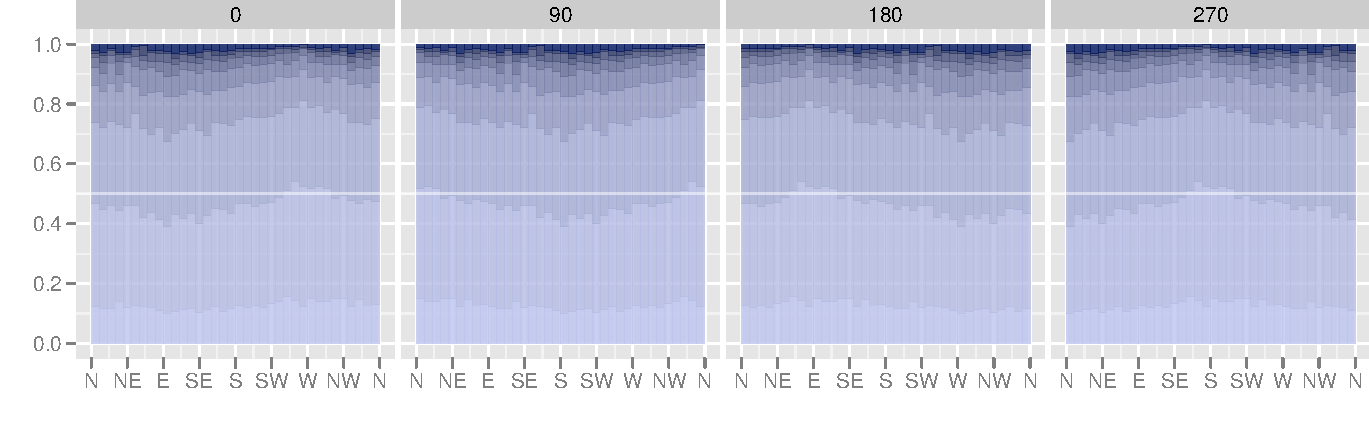
\includegraphics[width=\linewidth]{euclid-offset} 
   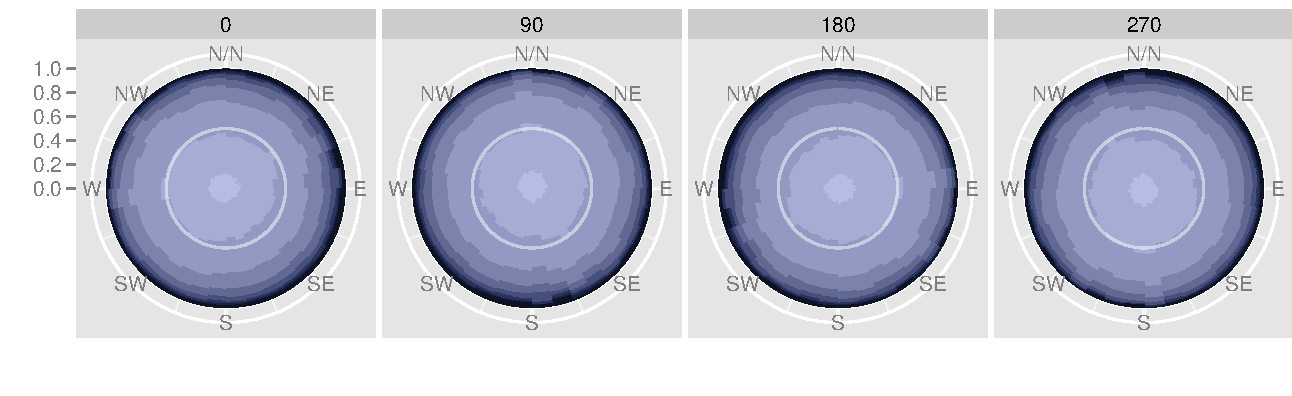
\includegraphics[width=\linewidth]{polar-offset} 
   \caption{ \label{fig:offset} (Top) Euclidean charts of the same sample, with shifts in wind direction by 90, 180, and 270 degrees. The shift by 90 and 270 leads to a `valley' versus a `mountain' pattern, whereas a shift by 180 degrees inverts the wave pattern from `down-up' to `up-down'.\hfill\newline
      (Bottom) Shifts in wind direction in the polar chart lead to rotations of the display by 90 degrees.}
\end{figure}

 This results in a shift of the wave in Euclidean charts and a rotation in the polar charts as can be seen in figure \ref{fig:offset}. Our initial hypothesis was that this would have no effect on the polar charts, but might have a deteriorating effect on the Euclidean charts, in the case that the peak or the valley of the wave was at either end of the $x$ axis. 
While these simple perturbations and different sample sizes allow us to get insight into different aspects of the designs, they also allow us to get multiple responses from each observer to assess individual ability without the need to go outside the framework of the original data, i.e. we leave the joint relationship between $x$ and $y$ essentially unchanged. For all of these combinations we produced two replicates, resulting in a total of 192 different lineups ($ 4 \text{ designs} \times 6 \text{ sample sizes} \times 4 \text{ offsets} \times 2 \text{ reps})$.

Data was collected using Amazon's Mechanical Turk (MTurk) service. XXX More details: website and screen shot.
 Each participant was shown ten lineups. In order to avoid people `gaming the system' as found in earlier studies \cite{heer:2010, kosara:2010}, participants were shown two specially prepared lineups as a baseline of performance -- if participants got just one of these two reference lineups correct, we required at least an overall correct percentage of 20\%, which is indicative of a performance that is better than guessing. Table \ref{tbl:treatment} gives an overview of the number of times lineups in each combination of design and sample size were shown, and in how many of them the data plot was correctly identified. 

\begin{table}[hbtp]
\resizebox{\linewidth}{!} {
	\rowcolors{1}{white}{lightgray}
	\begin{tabular}{ll|@{}r|@{}r|@{}r|@{}r|@{}r|@{}r}
	\multicolumn{2}{l}{sample size (in percent)}  & 2 & 4 & 6 & 8 & 10 & 24 \\ [1pt] \hline
	Polar & with & 13/49& 9/43 & 9/39 & 7/35 & 8/40 & 13/38 \\
	& without & 6/51&   4/34 &  5/34 &  6/39 & 11/43 &  12/37\\ [1pt] \hline
	Euclidean & with &12/24& 18/27 & 42/44 & 33/41 & 39/43 & 46/47\\
	& without & 13/41 &24/32& 39/44 & 47/51 & 40/45 & 34/37\\
	\end{tabular}
	}
\caption{\label{tbl:treatment} Breakdown of lineups: correct/shown. Each participant was shown eight lineups from the set above and two separate `test' charts.}
\end{table}

Besides correctness of responses, two additional response variables were recorded:  time taken for answer and a (subjective) confidence level, ranging from 1 (lowest) to 5 (highest), assessing how convinced participants are of the correctness of their answer. 
Figure \ref{fig:time} shows time taken until a decision was made in histograms, facetted by design and colored by correctness of answer. because of the skewness of the distributions, times were log-transformed. Polar charts take on average more time to answer, but are answered with much lower precision. Figure \ref{fig:conf} shows two barcharts of confidence levels by task, again coloring is used for correctness of answers. Euclidean displays lead to a very bimodal distribution of confidence: participants are either very sure or not sure at all of their answer. Confidence levels in polar charts are distributed much more uniformly.

\begin{figure}[htbp] %  figure placement: here, top, bottom, or page
   \centering
   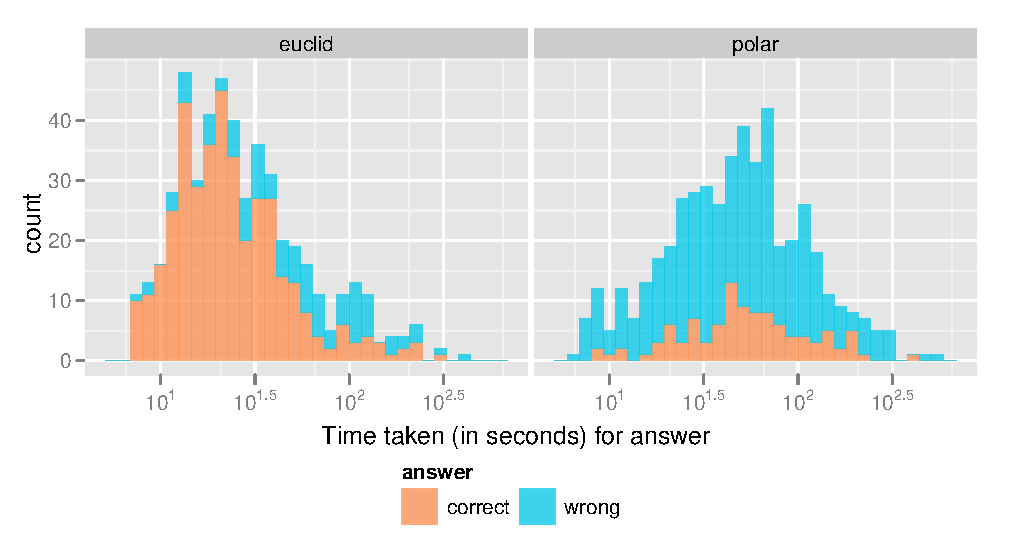
\includegraphics[width=\linewidth]{time-answer} 
   \caption{Histograms of time taken for answering lineups. On average the Euclidean design is answered faster and with higher power (percentage of correct answers). }
   \label{fig:time}
\end{figure}

\begin{figure}[htbp] %  figure placement: here, top, bottom, or page
   \centering
   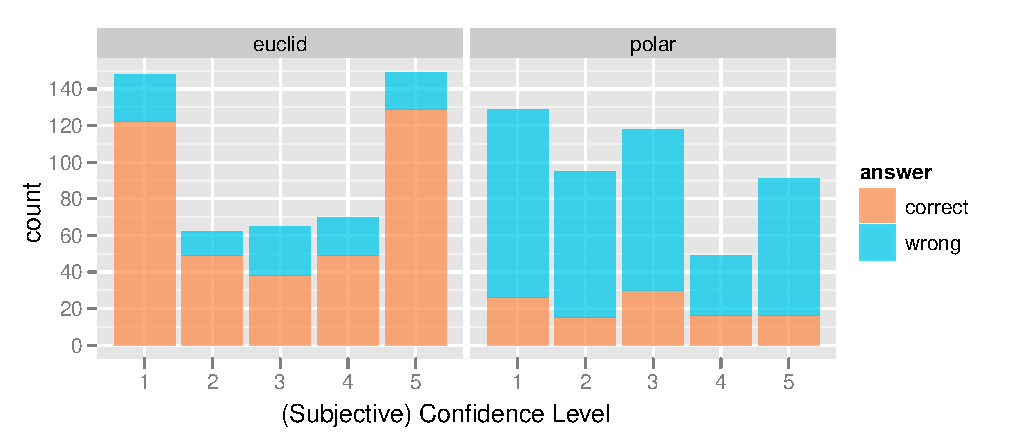
\includegraphics[width=\linewidth]{conf-answer} 
   \caption{Barcharts of (subjective) confidence in answering correctly for each lineup. A strongly bimodal distribution is apparent, while confidence levels for polar charts are more uniform. There are only slight (and non significant) difference between confidence levels and correctness of results.}
   \label{fig:time}
\end{figure}


Most generally this experiment can be paralleled to the pie chart versus barchart discussion \cite{***}. 
The Euclidean coordinate plot is made up of bars where areas are colored proportionally according to percentages. The polar coordinate plot is made up of pie slices which are also colored proportionally according to the data. 
Viewers of these charts will visually decode the areas of the bars and pie slices and make a judgement based on their decoding. According to  \citet[page=40]{kosslyn:2006}, area is usually perceived as a function of what the actual area is. This function is the area raised to an exponent of approximately 0.8 and then multiplied by a constant. However, when bars are parallel, the relative height of these bars is perceived very accurately. From this information, one could infer that the Euclidean coordinate plot may gain efficiency based on the height of the colored bars. 


For evaluating the results, we are using a linear mixed effects modeling \cite{pinheiro:2000} approach in all three of our response values, using the {\t R} package {\tt lme4} \cite{bates:2011}. 


Overall discussion: huge difference in power between polar charts and Euclidean, reference line has surprisingly little influence, but more so for polar charts than for barcharts,
An increase in sample size has positive impact on correctness (see figure \ref{fig:treatment} for an overview). Polar charts need much bigger sample size to see an increase in power -- only at about 24\% of the original data do we see about the same power as for Euclidean charts of a sample size of 2\%.
The offset changes are significant -- interestingly, borderline behavior (90 and 270 degrees) does not show a difference between polar and Euclidean charts, whereas an inversion of the wave pattern (first up, then down), does show a difference. Polar charts benefit more from this inversion than barcharts. This is an unexpected finding, but is consistent throughout different lineups in the data.

Time taken to answer was log transformed before the modeling process to de-emphasize the impact of very large values (up to 500 sec). The findings are consistent with correctness - time taken shows big differences between polar and Euclidean charts. The reference lines seem to increase the evaluation time, but not significantly. An increase in sample size decreases evaluation time, The inversion of the wave pattern at 180 degrees leads to a significant increase in time for Euclidean charts, but not for polar charts (at least not significantly). 

 Confidence levels are measured on a five point scale --- they are subjective assessments by the participant `how certain are you'. We model the value using a normal distribution - a discrete uniform distribution  might be more appropriate,
While there is a difference between the designs - participants reported higher confidence in dealing with the barcharts -- this is only  a trend (i.e. not significant at 5\% but below 10\%). The only significant effect on confidence level is visible for the use of reference lines in polar coordinates: participants report an increase in confidence when using the reference line (however, as we have seen before, this is not matched by an increase in actual correctness of the results).

\begin{table}[ht]
\begin{center}
\resizebox{\linewidth}{!} {
\rowcolors{2}{white}{lightgray}
\begin{tabular}{rrrrr}
  \hline
 & Estimate & Error & $z$-value & $p$-value \\ 
  \hline
euclid & -0.08 & 0.39 & -0.21 & 0.84 \\ 
polar & -1.98 & 0.32 & -6.13 & 0.00 \\ [1pt]
  reflineTRUE & -0.14 & 0.26 & -0.53 & 0.59 \\ [1pt]
  sample\_size & 0.27 & 0.04 & 6.31 & 0.00 \\ [1pt]
  offset 90 & -0.43 & 0.37 & -1.18 & 0.24 \\ 
  offset 180 & -0.89 & 0.35 & -2.51 & 0.01 \\ 
  offset 270 & 0.21 & 0.38 & 0.55 & 0.58 \\ [1pt]
  polar:reflineTRUE & 0.51 & 0.35 & 1.44 & 0.15 \\ [1pt]
  polar:sample\_size & -0.23 & 0.05 & -5.02 & 0.00 \\ [1pt]
  polar:offset 90 & 0.64 & 0.49 & 1.30 & 0.20 \\ 
  polar:offset 180 & 0.91 & 0.47 & 1.92 & 0.05 \\ 
  polar:offset 270 & -0.73 & 0.54 & -1.35 & 0.18 \\
   \hline
\end{tabular}}
\end{center}
\caption{\label{tbl:correct} Model output for correct result. }
\end{table}


\begin{table}[ht]
\begin{center}
\resizebox{\linewidth}{!} {
\rowcolors{2}{white}{lightgray}
\begin{tabular}{rrrrr}
  \hline
 & Estimate & Std. Error & $z$ value & $p$ value from multcomp\\ 
  \hline
(Intercept) & 3.58 & 0.09 & 41.34 \\ 
  test\_parampolar & 0.22 & 0.10 & 2.17 \\ 
  reflineTRUE & 0.08 & 0.06 & 1.50 \\ 
  sample\_size & -0.03 & 0.00 & -8.73 \\ 
  offset90 & -0.06 & 0.08 & -0.72 \\ 
  offset180 & 0.16 & 0.08 & 2.07 \\ 
  offset270 & -0.04 & 0.07 & -0.54 \\ 
  test\_parampolar:reflineTRUE & -0.03 & 0.08 & -0.40 \\ 
  test\_parampolar:sample\_size & 0.03 & 0.01 & 6.25 \\ 
  test\_parampolar:offset90 & 0.14 & 0.11 & 1.23 \\ 
  test\_parampolar:offset180 & -0.17 & 0.11 & -1.55 \\ 
  test\_parampolar:offset270 & 0.17 & 0.11 & 1.50 \\ 
   \hline
\end{tabular}}
\end{center}
\caption{\label{tbl:time} Model output for (log) time taken. }
\end{table}



\begin{table}[ht]
\begin{center}
\resizebox{\linewidth}{!} {
\rowcolors{2}{white}{lightgray}
\begin{tabular}{rrrr}
  \hline
 & Estimate & Std. Error & t value \\ 
  \hline
(Intercept) & 3.58 & 0.09 & 41.34 \\ 
  test\_parampolar & 0.22 & 0.10 & 2.17 \\ 
  reflineTRUE & 0.08 & 0.06 & 1.50 \\ 
  sample\_size & -0.03 & 0.00 & -8.73 \\ 
  offset90 & -0.06 & 0.08 & -0.72 \\ 
  offset180 & 0.16 & 0.08 & 2.07 \\ 
  offset270 & -0.04 & 0.07 & -0.54 \\ 
  test\_parampolar:reflineTRUE & -0.03 & 0.08 & -0.40 \\ 
  test\_parampolar:sample\_size & 0.03 & 0.01 & 6.25 \\ 
  test\_parampolar:offset90 & 0.14 & 0.11 & 1.23 \\ 
  test\_parampolar:offset180 & -0.17 & 0.11 & -1.55 \\ 
  test\_parampolar:offset270 & 0.17 & 0.11 & 1.50 \\ 
   \hline
\end{tabular}
}
\end{center}
\caption{\label{tbl:confidence} Model output for confidence level. }
\end{table}

\begin{figure*}[htbp] %  figure placement: here, top, bottom, or page
   \centering
   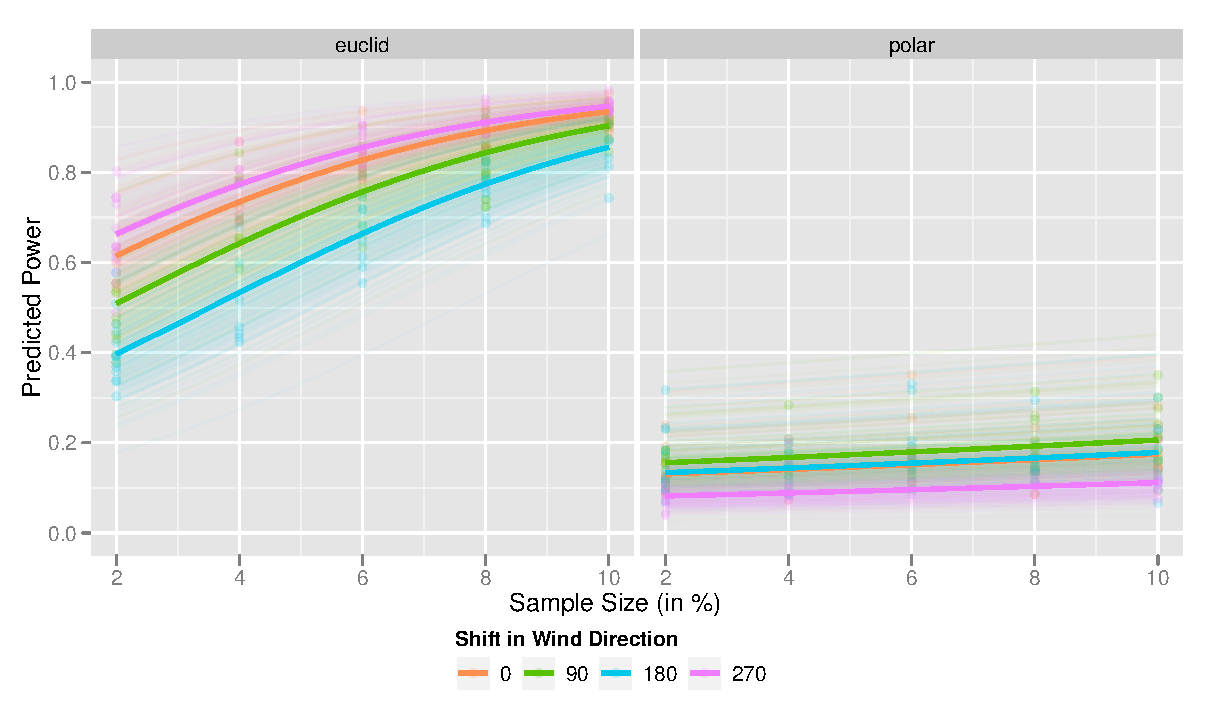
\includegraphics[width=\linewidth]{predict-power} 
   \caption{Predicted Power of designs.  The thin lines and the points on $y$ axis show  variability due to individuals' abilities. The saturated lines show average predicted power for each of the designs.}
   \label{fig:power}
\end{figure*}

The goal of this experiment is to understand the efficiency of displaying information using euclidian and polar coordinates. Efficiency is the deviation from independence, which can be simulated by taking permutations of the original dataset. Data concerning wind patterns and time between flights at SEA airport is used for these charts. The lineup chart is composed of 20 graphics with all of the exact same characteristics except for the data. One of the 20 graphics will be using original airport data while the other 19 will be permutations of that data. Efficiency of the chart types can be inferred by how accurately individuals pick out the plot with the original data. There are other variables which are introduced to further our understanding of the way we perceive euclidian and polar coordinates. All combinations of each level of the variables are involved in the experiment for both polar and euclidian coordinates. The graphics in each chart will all have exactly the same level of the variables with the only difference being the data. 

The other variables which are monitored are existence of reference line, placement of x-axis, and sample size. It is possible that one of the chart types benefits more from additional components such as reference lines. The polar and euclidian null charts will be shown either with or without a white reference line. The line is placed at slightly over 50 percent of the y axis. Additionally, the x-axis has four placements. The original dataset contains a characteristic wave pattern, which for euclidian coordinates, may be a large factor contributing to the perceived effectiveness of the graphic. Characteristic patterns such as the wave pattern may be perceived in a different way when viewed in polar coordinates. When the x-axis is is shifted the look of the pattern changes. The wave pattern is broken up for euclidian coordinates but for polar coordinates is only shifted around the axis. Finally, the amount of information necessary for detection as well as correctness is a measure for efficiency of the charts so the sample size which was taken from the original dataset is of interest. The original data set contained XXX,XXX observations from which 2, 4, 6, 8, 10, and 24 percent of the observations were sampled. Small sample sizes are easier to obtain because of time and money constraints. It would be nice to know if there is one type of chart which can show data trends using less information. 


 All combinations of these variables were repeated for plots with a reference line and without a reference line, as shown in figure \ref{layouts}.This figure shows examples of graphics showing the actual data, which in the experiment would be randomly positioned among 19 null plots. In total there are XXX unique charts which represent all different combinations of sample size, coordinate type, x-axis placement, and whether or not there is a reference line. The charts are all assigned a difficulty level, which is based on sample size, on a scale from zero to four. There are two plots assigned a difficulty level of zero. These two charts, one polar and one Euclidian, were made from computer generated data and intended to be at the level where an individual, if he or she is not purely guessing, should be able to find the correct plot. 


Amazon's Mechanical Turk is an online service in which individuals can request and perform simple tasks and surveys for money. Using Turk we were able to gather data on how people responded to the charts. Each person is shown a series of ten charts and asked to choose the graphic on each chart which they think is "different". They then identify, from a list of choices, why they chose this particular chart as well as how confident they are on a scale of one to five. Personal information such as age group, gender, and education is also collected on a voluntary basis. The amount of time it took the individual to answer is also recorded. This study allows us to make informed judgments about how the plot type effects efficiency in terms of accuracy and time spent reading the plots. Xcite stephen few?X

Effect is deviation from independence. Cannot be properly measured statistically except in highly aggregated situations, where the effect might be washed out.

%Most generally this experiment can be paralleled to the pie chart versus barchart discussion. The Euclidian coordinate plot is made up of bars *whose?* areas are colored proportionally according to the data. The polar coordinate plot is made up of pie slices which are also colored proportionally according to the data. Viewers of these charts will visually decode the areas of the bars and pie slices and make a judgement based on their decoding. How accurate this judgment is is left to be discussed. According to  \citet[page=40]{kosslyn:2006}, area is usually perceived as a function of what the actual area is. This function is the area raised to an exponent of approximately 0.8 and then multiplied by a constant. However, when bars are parallel, the relative height of these bars is perceived very accurately. From this information, one could infer that the Euclidian coordinate plot may gain efficiency based on the height of the colored bars. 


Pie versus Barchart discussion is pretty old: cite some of the literature:

From Stephen Few, perceptual edge:
	When a graph is made, quantitative and categorical information is encoded by a display method. Then the information is visually decoded. This visual perception is a vital link. No matter how clever the choice of the information, and no matter how technologically impressive the encoding, a visualization fails if the decoding fails. Some display methods lead to efficient, accurate decoding, and others lead to inefficient, inaccurate decoding. It is only through scientific study of visual perception that informed judgments can be made about display methods. (William S. Cleveland, The Elements of Graphing Data, Hobart Press, 1994, p. 1)
	
	The systematic distortion of area is captured by �Steven�s Power Law,� which states that the psychological impression is a function of the actual physical magnitude raised to an exponent (and multiplied by a scaling constant). To be precise, the perceived area is usually equal to the actual area raised to an exponent of about 0.8, times a scaling constant...In contrast, relative line length [such as the lengths of bars] is perceived almost perfectly, provided that the lines are oriented the same way \cite[page=40]{kosslyn:2006}
	
	
	We make angle judgments when we read a pie chart, but we don�t judge angles very well. These judgments are biased; we underestimate acute angles (angles less than 90�) and overestimate obtuse angles (angles greater than 90�). Also, angles with horizontal bisectors (when the line dividing the angle in two is horizontal) appear larger than angles with vertical bisectors. (Naomi Robbins, Creating More Effective Graphs, Wiley, 2005, p. 49)
	
	 Edward Tufte once said that �the only worse design than a pie chart is several of them, for then the viewer is asked to compare quantities located in spatial disarray both within and between pies� (Edward Tufte, The Visual Display of Quantitative Information, Graphics Press, 1983, p. 178.)

 We do not claim to settle the question - which is multi-facetted and will not have a clear 'winning' design but instead very much depends on the purpose of the chart and task at hand.

